%!TeX root = Chapter_ComputationalMethods
\documentclass[../../CompleteThesis/Complete_1stDraft.tex]{subfiles}

\begin{document}

\section[Splines and Interpolation]{Splines and Interpolation}	
\label{Sec:CompMeths_SplinesAndInterpolation}
\subsection[Interpolation][Interpolation]{Interpolation}
\label{Subsec:CompMeths_SplinesAndInterpolation_Interpolation}
Interpolation is a tool that can be used - and misused - to extract more information out of a given set of data. Used correctly, interpolation can reveal more information than is initially available and disclose connections not apparent at first, but used incorrectly, it can be manipulated to infer misleading correlations and lead to inaccurate conclusions. Thus it is a tool that must be used with care. Aiming to avoid incorrect deductions and inferences one should at first gain as much knowledge about the data at hand as possible. By understanding how the data have come about and gaining knowledge about the underlying physical theories a somewhat deficient data set can robustly and securely be interpolated to accommodate the needs of the analysis. In the case of this thesis, both knowledge about data gathering and the physics at play have been gained and thus some of the common fallacies may be avoided. The limits of the data available is due to the discrete sampling, leading to a minimum sampling of about 26 samples per meter of ice.
When considering that the depth series of 32 years between Tambora and Laki is just above 10 meters, this means that each meter of ice needs to contain at least three years on average. 26 samples per three years might not sound as a bad sampling interval, but if the goal is to show seasonality and give a best estimate of annual layer thickness, interpolation could be put to good use to be able to give better estimates of the exact placement of peaks and valleys.\\

\textbf{Existence, Uniqueness and Conditioning}\\
Considering any attempt to create an interpolant to fit a number of data points, the questions of uniqueness and existence is a matter of matching the data points with the number of parameters in the interpolant. If there are too few parameters, the interpolant does not exist, as it will not pass through all data points. If there are too many, the interpolant will not be unique. Formally this can be described through a system of linear equations.\\
For any data set consisting of $(t_i, y_i),\; i=1,...,m$ points, an interpolant can be chosen from a function space spanned by some suitable set of basis functions, $\phi_1(t),...,\phi_n(t)$. The interpolant can then be described as a linear combination of these basis functions:
\begin{equation}
	f(t) = \sum_{j=1}^{n} x_j\phi_j(t)
\end{equation}
The interpolant can then be found by determining the parameters $x_j$ by requiring that the interpolant $f$ must pass through the $M$ data points $(t_i,y_i)$:
\begin{equation}
	f(t_i) = \sum_{j=1}^{n} x_j\phi_j(t_i) = y_i, \quad i=1,...,m
\end{equation}
This can of course also be written compactly in matrix form as a system of linear equations:
\begin{equation}
	\boldsymbol{A}\boldsymbol{x}=\boldsymbol{y}
\end{equation}
In this equation $\boldsymbol{A}$ is the $m\times n$ basis matrix, which entries consists of the value of the $n$ basis functions evaluated at the $m$ data points, $a_{ij}=\phi_j(t_i)$, the $m$ vector $\boldsymbol{y}$ consists of the known data values $y_i$, and the $n$ vector $\boldsymbol{x}$ consists of the unknown, to be determined, parameters $x_j$.\\
From linear algebra we know, that if we choose the number of basis function ot be equal to the number of data points, $n=m$, the basis matrix will be square, and thus - given the matrix is nonsingular - the system will be determined, and the data points can be fit exactly. Though in some problems it is beneficial to choose the system to be either overdetermined(less parameters than data points, the data cannot be fit exactly) or underdetermined(more parameters than data points, giving freedom to allow satisfaction of additional properties or conditions).\\ 
So the existence and uniqueness of an interpolant is given by the non-singularity of the basis matrix, be it square or not and the conditioning of the matrix points to the parameters' sensitivity to perturbations. An ill-conditioned basis matrix will lead to high sensitivity in the parameters, but this problem can still be approximately solvable through Gaussian elimination with partial pivoting, but this solution will mean that the coefficients may be poorly determined.

\subsubsection[Polynomial]{Polynomial Interpolation}
\label{Sec:CompMeths_SplinesAndInterpolation_Interpolation_Polynomial}
The most common way to determine an interpolant is through polynomials. Denoting a set of all polynomials of degree at most $k,\quad k\geq 0$ as $\mathbb{P}_k$, it can be seen that this set forms a vector space of dimension $k+1$. The basis functions that span this vector space can be chosen to be composed of a number of different functions and this choice has a great influence on both the cost of computation and manipulation of the interpolant, and the sensitivity of the parameters, i.e. the conditioning of the basis matrix. \\
Considering $n$ data points it is obvious to choose $k=n-1$ so that the dimension of the vector space matches the number of data points. The maybe most natural choice of basis for $\mathbb{P}_{n-1}$ is one that consists of the first $n$ monomials\footnote{Roughly speaking, a polynomial with only one term.},
\begin{equation}
	\phi_j(t) = t^{j-1},\quad j=1,...,n.
\end{equation}
Thus any given polynoial $p_{n-1}\in\mathbb{P}_{n-1}$ will be of the form 
\begin{equation}
	p_{n-1}(t)=x_1 + x_2t + \cdots+x_n t^{n-1}.
\end{equation}
In this basis the system of $n\times n$ linear equations will be of the form 
\begin{equation}
	\boldsymbol{A}\boldsymbol{x} = 
	\begin{bmatrix}
		1 & t_1 & \cdots & t_1^{n-1}\\
		1 & t_1 & \cdots & t_1^{n-1}\\
		\vdots & \vdots & \ddots & \vdots \\
		1 & t_1 & \cdots & t_1^{n-1}\\
		
	\end{bmatrix}
	\begin{bmatrix}
		x_1\\
		x_2\\
		\vdots\\
		x_n
	\end{bmatrix}
	=
	\begin{bmatrix}
		y_1\\
		y_2\\
		\vdots\\
		y_n
	\end{bmatrix}
	= \boldsymbol{y}.
\end{equation}
This type of matrix with geometric progression, i.e. the columns are successive powers of some independent variable $t$ is called a \todo{COMP-INTERP: REFERENCE!!!}Vandermonde matrix. \\
When using the monomial basis and using a standard linear equation solver to determining the interpolants coefficients requires $\mathcal{O}(n^3)$ work and often results in ill-conditioned Vandermonde matrices $\boldsymbol{A}$, especially for high-degree polynomials. This ill-conditioning is due to the monomials of higher and higher degree being more and more indistinguishable from each other. This makes the columns of $\boldsymbol{A}$ nearly linearly dependent, resulting in almost singular matrices, and thus highly sensitive coefficients. For high enough $n$, the Vandermonde matrix becomes efficiently singular, to computational precision at least, though, as mentioned, this can be worked around, but requires some additional computational work. 

\begin{marginfigure}
	\centering
	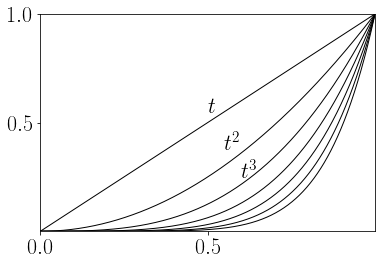
\includegraphics[width=\marginparwidth]{Monomials.png}
	\caption[Monomials]{\footnotesize{Illustration of the first eight monomials.}}% Black is the measured densities during drilling, blue is the modelled density profile given a Herron Langway model, and orange is a Herron Langway model with a criterion to minimize the distance to the actual measurements.}}
	\label{fig:Monomials}
\end{marginfigure}
\subsubsection[Piecewise Polynomial]{Piecewise Polynomial Interpolation and Splines}
\label{Sec:CompMeths_SplinesAndInterpolation_Interpolation_PiecewisePolynomial}
The amount of work needed to solve the system as well as the conditioning of the system can be improved by using a different basis all together. Some different bases superior to the monomial that are worth mentioning are the Lagrange basis functions, the Newton basis functions and the orthogonal polynomials\todo{COMP-INTERP: REFERENCES!!}. But for this thesis we take a step further into the interpolation theory, as the choice of basis functions might not be enough to work around some of the problems connected with fitting a single polynomial to a large number of data points(i.e. oscillatory behaviour in the interpolant, nonconvergence or issues around the boundaries).\\
These practical and theoretical issues can be avoided through the use of piecewise polynomial interpolation, with the advantage that a large number of data points can be fitted with low-degree polynomials. \\
When turning to piecewise polynomial interpolation of the data points $(t_i,y_i),\quad i=1,...,n$, $t_1 < t_2 < \cdots < t_n$, a different polynomial is chosen for each subinterval $[t_i,t{i+1}]$. Each point $t_i$, where the interpolant changes is called knots or control points. The simplest piecewise interpolation is piecewise linear interpolation, where each knot is connected with a straight line. If we consider this simple example it appears that by eliminating the problems of nonconvergence and unwanted oscillatory behaviour, the smoothness of the interpolant is sacrificed. This might be true for this simplistic example but since there are a number of degrees of freedom in choosing each piecewise polynomial interpolant, the smoothness can be reintroduced by explotiting a number of these measures. One way of doing this is by demanding knowledge of both the values and the derivatives of the interpolant at each data pint. This just adds more equations to the system, and thus to have a well-defined solution, the number of equations must match the number of parameters. This type of interpolation is known as Hermite interpolation. The most common choice for this interpolation, to still maintain simplicity and computational efficiency, is cubic Hermite interpolation. This introduces a piecewise cubic polynomial with $n$ knots, and thus $n-1$ interpolants each with 4 parameters to fit, leading to $4(n-1)$ parameters to be determined. Since each of the $n-1$ cubics must match the data points at each end of the subinterval, it results in $2(n-1)$ equations, and requiring the derivative to be continuous, i.e. match at the end points, an additional of $n-2$ equations are taken in. This leads to a system consisting of $2(n-1) + (n-2) = 3n - 4$ equations to fit to the $4n - 4$ parameters. This leaves $n$ free parameters, meaning that a cubic Hermite interpolant is not unique and the remaining free parameters can be used to accommodate further or additional constraints that might be around the problem at hand. \\\newline
\indent \textbf{Cubic Spline Interpolation}\\
One way of using the remaining free parameters is by introducing \textit{splines}\marginpar{\footnotesize A spline is a piecewise polynomial of degree $k$ that is continuously differentiable $k-1$ times.}. A cubic spline is, given the spline definition, a piecewise cubic polynomial, a polynomial of degree $k=3$, and must then be $k-1 = 2$ times differentiable. Thinking back on the Hermite cubic, we were left with $n$ free parameters. By demanding continuity of also the second derivative, we introduce $n-2$ new parameters, leaving only 2 final parameters to be free. These 2 remaining parameters can be fixed through a number of different requirements, e.g. by forcing the second derivative at the endpoints to be zero, which leads to the \textit{natural} spline.\\
The Hermite and spline interpolations are useful for different cases. The Hermite cubic might be more appropriate for preserving monotonicity if it is known that the data are monotonic. On the contrary, the cubic spline may enforce a higher degree of smoothness as it takes the second derivative into account as well.\\
For the case of this study, cubic spline interpolation is used to either evenly redistribute slightly unevenly sampled data or to enhance resolution for more precise peak detection. The general method for cubic spline interpolation used here is described in the following.

Assuming the original depth array $\text{\textbf{d}}$ is distributed as $d_{i-1} < d_i < d_{i+1}$ with $i = 0, ..., n-1$ has a minimum sampling distance as $\Delta_{\text{min}}$ we define the new sampling distance for the new depth array $\hat{\text{\textbf{d}}}$ as $\Delta =\Delta_{\text{min}}$ - again assuming that $\hat{\text{\textbf{d}}}_{j-1} < \hat{\text{\textbf{d}}}_j < \hat{\text{\textbf{d}}}_{j+1}$ with $j = 0, ..., \hat{n}-1$. This makes it possible to define the first and last value of the new array as
\begin{equation}
	\hat{\text{d}}_0 = \Delta \lceil \frac{\text{d}_0}{\Delta}, \rceil 
	\label{Eq:InterpDepthMin}
\end{equation}
\begin{equation}
	\hat{\text{d}}_{\hat{n}-1} = \Delta \lfloor \frac{\text{d}_{n-1}}{\Delta} \rfloor.
	\label{Eq:InterpDepthMax}
\end{equation}
From this the number of values in the new array, $\hat{n}$, can be determined as
\begin{equation}
	\hat{n} = 1 +  \frac{\hat{\text{d}}_{\hat{n}-1} - \hat{\text{d}}_0}{\Delta},\;\;\;\;\; \hat{n} \in\mathbb{Z}.
\end{equation}
Thus our new depth array will be given as
\begin{equation}
	\hat{\text{\textbf{d}}} = \hat{\text{d}}_0 + j\cdot\Delta,\;\;\;\;\; j = 0, ..., \hat{n}-1.
\end{equation}
The original data are then used to define a cubic spline interpolation function to which the redistributed depth data points can be matched. For this part of the data analysis the \lstinline[columns=fixed]|SciPy.interpolate| Python (REFERENCE) package with \lstinline[columns=fixed]|SciPy.interpolate.CubicSpline| for the cubic spline interpolation.

\subsection[Interpolation in this Project][Interpolation in this Project]{Cubic Spline Interpolation in this Project}
\label{Subsec:CompMeths_SplinesAndInterpolation_InterpolationInThisProj}
For this project cubic spline interpolation has been implemented and examined in two particular sections of the analysis: 
\begin{enumerate}
	\item Cubic spline interpolation of raw, uneven data to represent even data, that can be analyzed through fast spectral transforms.
	\item Cubic spline interpolation of the final back-diffused signal estimate to enhance resolution for more efficient peak detection.
\end{enumerate}

\subsubsection[Interpolation 1]{Interpolation of Data Before Deconvolution}
\label{Subsubsec:CompMethod_StabilityTests_Interpolation1}

The first interpolation is needed, if the fast spectral transforms FFT or FCT are used, as one of the conditions of the algorithms is that the data are evenly spaced. At first, this was implemented in the analysis, but this had the risk of excluding some information that might lie in the unevenly sampled data. Later, the method was abandoned in favor of implementing a nonuniform spectral transform (NUFT or NDCT), which is slower than the FFT and FCT, but carries all information from the unevenly sampled signal into the spectral domain. Luckily, this nonuniform transform needs only be carried out once, as the inverse transform, i.e. resampling in time domain, can be done uniformly without loss of information and any future spectral transforms can then be performed through FFT or FCT.
Even though the first interpolation method was later abandoned, some analysis was carried out with it to examine the effect of the size of the resampled, interpolated data on the final diffusion length estimate. Examples of a resampled signal can be seen in Figure \ref{Fig:COMPMETH_SiteA_DataSplineInterp} and Figure \ref{Fig:COMPMETH_SiteA_MultiSplineInterp}. Figure \ref{Fig:COMPMETH_SiteA_MultiSplineInterp} shows how sample resolution affects information from the signal. The higher sampling resolution, the more information is retained. But higher sampling resolution also means more data to be analyzed, which might slow down any analysis algorithms developed. This might create some headache if an entire ice core length of a couple thousand meters should be examined, but for this study only af few meters are of interest, and thus it should not create delays in the computation time.

\begin{figure}[h]
	\centering
	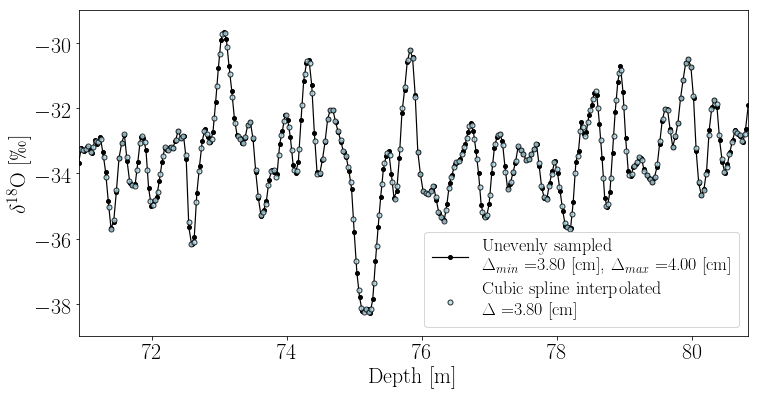
\includegraphics[width=\textwidth]{SiteA_DataSplineInterp.png}
	\caption{Unevenly sampled signal from Site A resampled using cubic spline interpolation to an even signal with a new sample size equal to the minimum sample size found in the raw signal.}
	\label{Fig:COMPMETH_SiteA_DataSplineInterp}
\end{figure}

\begin{figure}[h]
	\centering
	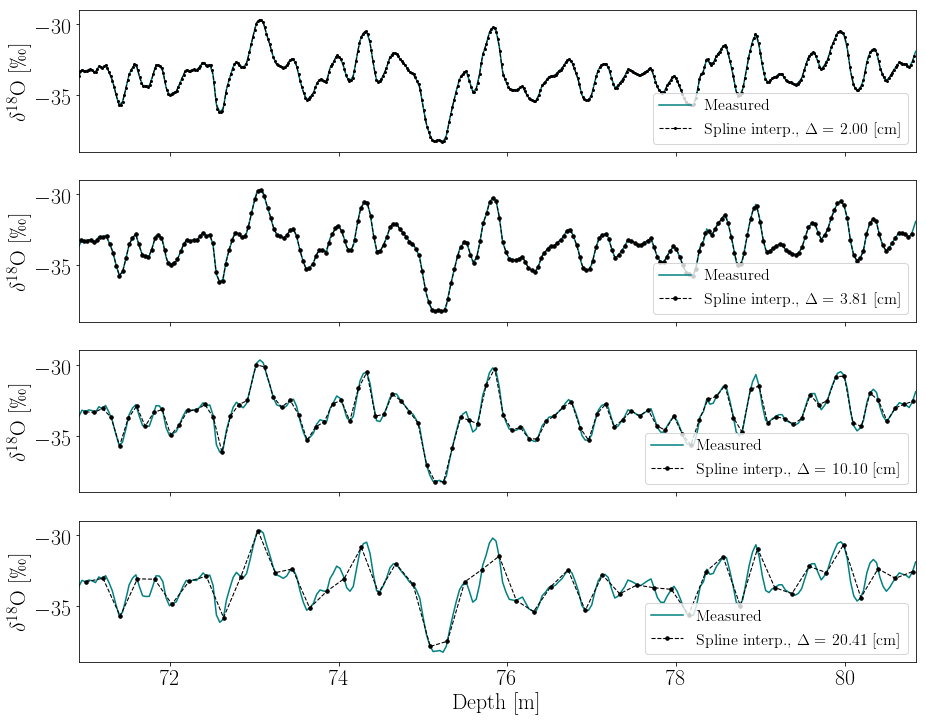
\includegraphics[width=\textwidth]{SiteA_MultiSplineInterp.png}
	\caption{Four different resampled signals of Site A data, showing loss of information when resampling resolution is low.}
	\label{Fig:COMPMETH_SiteA_MultiSplineInterp}
\end{figure}

To examine the effect of the resampling resolution on the final diffusion length estimate when conducting a spline interpolation before carrying out the back-diffusion, the full diffusion length analysis has been performed with 100 new interpolation resampling sizes in the range $[\Delta_{\text{min}};\Delta_{\text{max}}]$. This gives an idea of the stability of the method considering both sample size of the raw data and resampling by interpolation. The minimum and maximum interpolation samplings are presented in Table \ref{tab:InterpSamples} and an illustration of the test results can be seen in Figure \ref{Fig:COMPMETH_SamplingVsDiffLen_interpBF}.

\marginnote{%
	\footnotesize
	\centering
	\begin{tabular}{lcc}
		\toprule
		\textbf{Site} & $\Delta_{\text{min}}$& $\Delta_{\text{max}}$\\
		& [m] & [m] \\
		\midrule
		Crete & 0.02 & 0.13 \\
		Site A & 0.022 & 0.12 \\
		Site B & 0.01 & 0.14 \\
		Site D & & \\
		Site E & 0.02 & 0.12 \\
		Site G & 0.02 & 0.11 \\
		\bottomrule
	\end{tabular}
	\captionof{table}{\footnotesize Minimal and maximal new sample resolution used for testing interpolation before back-diffusion. Each test is run with 100 different new sample resolutions between $\Delta_{\text{min}}$ and $\Delta_{\text{max}}$.}
	\label{tab:InterpSamples}
}[0.5cm]%


\begin{figure}[h]
	\centering
	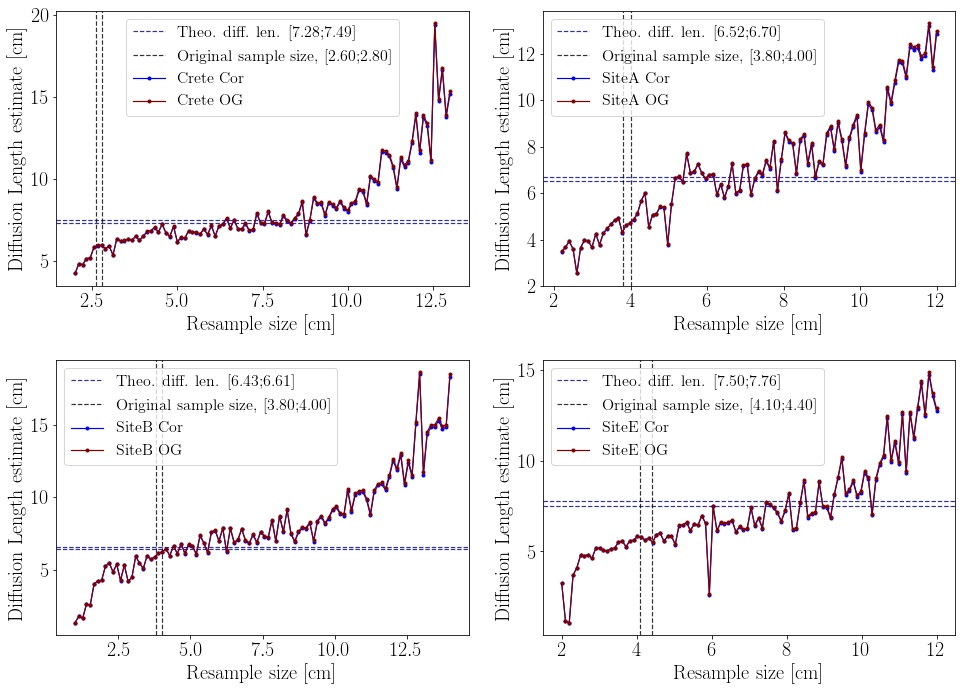
\includegraphics[width=\textwidth]{SamplingVsDiffLen_interpBF.jpg}
	\caption{}
	\label{Fig:COMPMETH_SamplingVsDiffLen_interpBF}
\end{figure}

\todo{COMPMETH: Write figure captions to all figures.}


\subsubsection[Interpolation 2]{Interpolation of Data After Deconvolution}
\label{Subsubsec:CompMethod_StabilityTests_Interpolation2}
The second interpolation is carried out after deconvoluting and back-diffusing the signal, but before detecting peaks. Splines are especially effective when trying to find features like peaks in data which underlying signal is continuous, smooth and differentiable, but the sampling is discrete and thus the data are discrete and non-smooth. The isotopic signal under examination here is assumed to be truly smooth and continuous throughout the core - unless any gaps are present. Thus the cubic spline interpolation is a good tool for estimating a higher resolution version of the final back-diffused data series to use for peak detection. This makes the detection of peaks and troughs more precise, as there might not be a discrete data point exactly at the top of a peak, but the spline interpolation then estimates where the most likely top of the peak must be, on the basis of the existing data. Examples of three different interpolation samplings are presented in Figure \ref{Fig:COMPMETH_SiteA_InterpAF_4samplings}. The effect of resampling after deconvolution on the final diffusion length estimate is illustrated in Figure \ref{Fig:COMPMETH_SamlingVsDiffLen}.

\begin{figure}[h]
	\centering
	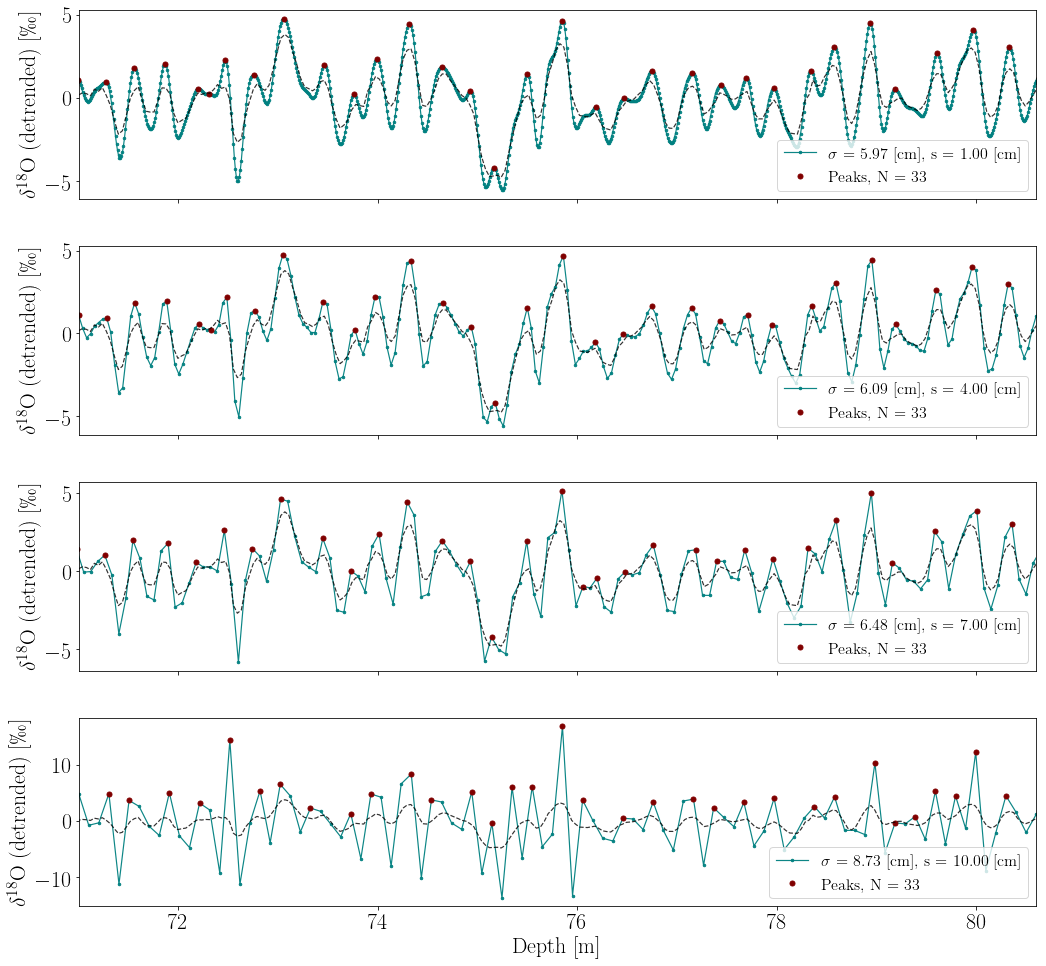
\includegraphics[width=\textwidth]{SiteA_InterpAF_4samplings.png}
	\caption{}
	\label{Fig:COMPMETH_SiteA_InterpAF_4samplings}
\end{figure}

\begin{figure}[h]
	\centering
	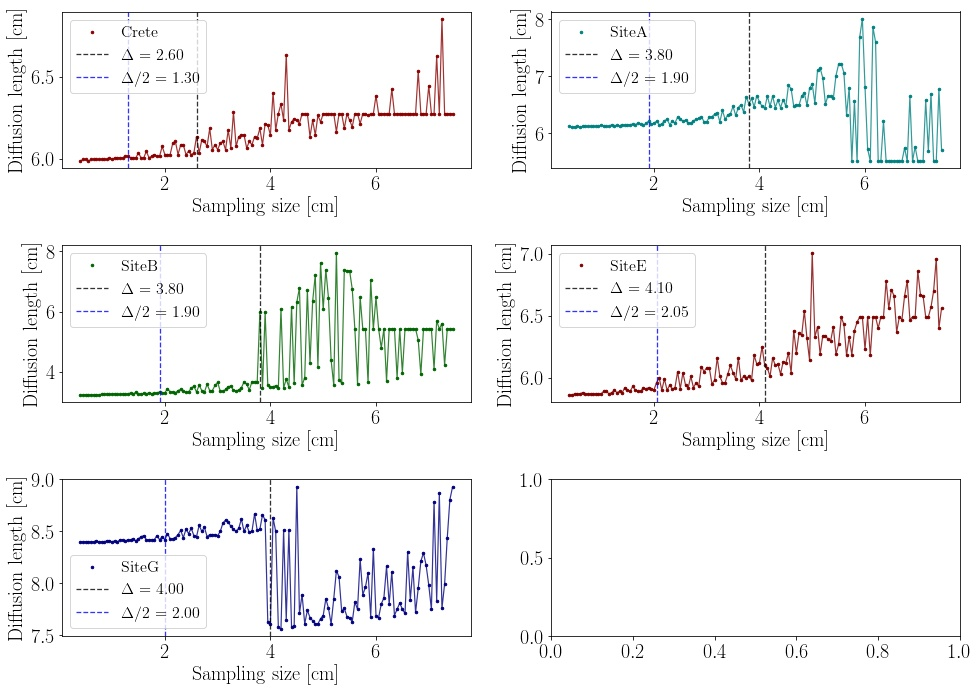
\includegraphics[width=\textwidth]{SamlingVsDiffLen.jpg}
	\caption{}
	\label{Fig:COMPMETH_SamlingVsDiffLen}
\end{figure}

\section[Peak Detection]{Peak Detection}
\label{Sec:CompMeths_PeakDetection}

Knowing that water isotopic data are a proxy for temperature, the most obvious way to determine annual layers in the signals is by detecting peaks and troughs. During colder periods, e.g. winter, the air masses arriving at the ice core sites have formed more precipitation before reaching the sites, and the vapor that results in this final precipitation is then more depleted of heavy isotopes, resulting in lower isotopic values, troughs in Figure \ref{Fig:ICE_Crete_10m_dated}. The precipitation falling during warmer conditions, e.g. summer, is correspondingly less depleted of the heavy isotopes, and results in higher isotopic values, peaks in Figure \ref{Fig:COMPMETH_Crete_10m_PeaksTroughs}.
\begin{figure}[h]
	\centering
	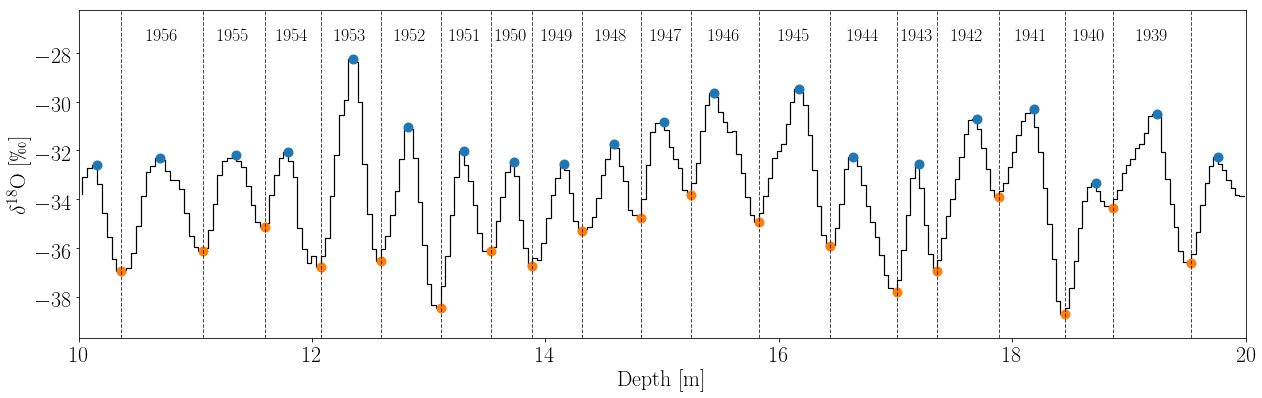
\includegraphics[width=\textwidth]{Crete_10m_PeaksTroughs.png}
	\caption{Ten meters of the top of Cretê ice core, with identification and dating of 19 annual layers, with peaks(blue) corresponding to summers and troughs(orange) corresponding to winters.}
	\label{Fig:COMPMETH_Crete_10m_PeaksTroughs}
\end{figure}
Peak detection and layer counting has previously been carried out by visual inspection of the ice core depth signals, but as computers and algorithms have become more integrated in data analysis, it is now more common to use different computational methods. Developing and implementing layer counting and peak detection algorithms can be done in a number of different ways, but for this project, at first a very simple method has been initially implemented and later the method has been improved and optimized through a number of different constraints. One could also use different pattern recognition techniques[REFERENCE]\todo{References here.} to achieve more intelligent detection, and later some of these methods will be presented.\\
The most naïve approach, and the one first implemented in this project, to peak detection is to simply find local maxima by comparing neighbouring values. When examining point $d_i$, the point is deemed a local maxima, if $d_{i\pm1} < d_i$. Local minima, troughs, can be found in exactly the same manner by finding minima as $d_{i\pm1} > d_i$. A very simple constraint for this method is to keep a required minimal distance between peaks, so that two peaks cannot be detected within a point distance of $\Delta d_{\text{min}}$. For example at a depth of 12 m in Figure \ref{Fig:COMPMETH_Crete_10m_PeaksTroughs} two troughs can be seen, but only one is chosen, as they are within the threshold distance to each other, which here is set to $\Delta d_{\text{min}} = 7$ points. Here, the lowest of the two troughs is chosen. The threshold distance can be chosen in different ways, for this short section it has been chosen through visual inspection, but more generally it can be chosen by examining some of the intrinsic properties of the signal, more about this in Section \ref{}.

\todo{COMPMETH-PEAKDET: Write about better peak detection with cubic spline interpolation (enhanced resolution)}


\section[Parallelization]{Parallelization}	
\label{Sec:CompMeths_Parallelization}
\todo{COMP-PARAL: Do some actual parallelization! And write this entire section}

\end{document}
